\documentclass[a4paper, 12pt]{abnt}

\usepackage[brazil]{babel}
\usepackage[T1]{fontenc}
\usepackage[utf8]{inputenc}
\usepackage{dsfont}
\usepackage{amssymb,amsmath}
\usepackage{multirow}
\usepackage[alf]{abntcite}
\usepackage[pdftex]{color, graphicx}
\usepackage{colortbl}
\usepackage{url}
\usepackage{abnt-alf}
\usepackage{abntcite}
\usepackage{algorithm}
\usepackage{algorithmic}
\usepackage{multicol}

\floatname{algorithm}{Algoritmo}
\renewcommand{\algorithmicrequire}{\textbf{Entrada:}}
\renewcommand{\algorithmicensure}{\textbf{Saída:}}
\renewcommand{\algorithmicend}{\textbf{fim}}
\renewcommand{\algorithmicif}{\textbf{se}}
\renewcommand{\algorithmicthen}{\textbf{então}}
\renewcommand{\algorithmicelse}{\textbf{senão}}
\renewcommand{\algorithmicfor}{\textbf{para}}
\renewcommand{\algorithmicforall}{\textbf{para todo}}
\renewcommand{\algorithmicdo}{\textbf{faça}}
\renewcommand{\algorithmicwhile}{\textbf{enquanto}}
\renewcommand{\algorithmicloop}{\textbf{loop}}
\renewcommand{\algorithmicrepeat}{\textbf{repetir}}
\renewcommand{\algorithmicuntil}{\textbf{até que}}
\renewcommand{\algorithmiccomment}[1]{\% #1}


\newcommand{\ignore}[1]{}


\hyphenation{PYTHON ou-tros}


\begin{document}

	\frenchspacing

	% Capa
% Proteção externa do trabalho e sobre a qual se imprimem as informações indispensáveis 
% à sua identificação.

% Especificação da capa
\begin{titlepage}
	\begin{center}
		
		% Cabeçalho (não deve ser modificado)
		% Contém o brasão da Universidade, o logotipo do Departamento, além dos dados
		% relacionados à vinculação do aluno (Universidade, Centro, Departamento e Curso)
		\begin{minipage}{2cm}
			\begin{center}
				
\includegraphics[width=1.7cm, height=2.0cm]{Imagens/Brasao-UFRN.jpg}
			\end{center}
		\end{minipage}
		\begin{minipage}{11cm}
			\begin{center}
				\begin{espacosimples}
					{\small \textsc{Universidade Federal do Rio Grande do Norte}			\\
							  \textsc{Centro de Ciências Exatas e da Terra}						\\
							  \textsc{Departamento de Informática e Matemática Aplicada}	\\
							  \textsc{Bacharelado em Engenharia de Software}}
				\end{espacosimples}
			\end{center}
		\end{minipage}
		\begin{minipage}{2cm}
			\begin{center}
				
\includegraphics[width=1.8cm, height=1.5cm]{Imagens/Logotipo-DIMAp.jpg}
			\end{center}
		\end{minipage}
			
		\vspace{5cm}
						
		% Título do trabalho
		{\setlength{\baselineskip}%
		{1.3\baselineskip}
		{\LARGE \textbf{Argue: uma ferramenta para escolha de bibliotecas no ecossistema Ruby}}\par}
			
		\vspace{4cm}
			
		% Nome do aluno (autor)
		{\large \textbf{Waldyr Guimarães Araújo de Souza}}
						
		\vspace{7cm}
		
		% Local da instituição onde o trabalho deve ser apresentado e ano de entrega do mesmo
		Natal-RN\\Dezembro 2015
	\end{center}
\end{titlepage}

	% Folha de rosto
% Contém os elementos essenciais à identificação do trabalho.

% Título, nome do aluno e respectivo orientador e filiação
\titulo{\Large{Argue: uma ferramenta de auxilio à escolha de bibliotecas no ecossistema Ruby}}
\autor{Waldyr Guimarães Araújo de Souza}
\orientador[Orientador]{\par Prof. Dr. Fernando Marques Figueira Filho}
\instituicao
{
	Universidade Federal do Rio Grande do Norte -- UFRN \par 
	Departamento de Informática e Matemática Aplicada -- DIMAp
}
	
% Natureza do trabalho (não deve ser modificada)
\comentario
{
	Proposta de Monografia de Graduação apresentada ao Departamento de Informática e Matemática Aplicada do 
	Centro de Ciências Exatas e da Terra da Universidade Federal do Rio Grande do Norte como
	requisito parcial para a obtenção do grau de bacharel em Engenharia de Software.
}
		
% Local e data
\local{Natal-RN}
\data{Dezembro de 2014}
	
\folhaderosto

	\begin{folhadeaprovacao}
	\setlength{\ABNTsignthickness}{0.4pt}
	\setlength{\ABNTsignwidth}{10cm}
	
	\noindent 
	Monografia de Graduação sob o título \textit{Título da monografia} apresentada por 
	Nome do aluno e aceita pelo Departamento de Informática e Matemática Aplicada do
	Centro de Ciências Exatas e da Terra da Universidade Federal do Rio Grande do Norte,
	sendo aprovada por todos os membros da banca examinadora abaixo especificada:
		
	\assinatura
	{
		Titulação e nome do(a) orientador(a)\\
		{\small Fernando Marques Figueira Filho PhD} 															\\ 
		{\footnotesize
			Departamento 																	\\
		  	Universidade
		}
	}
	
	\assinatura
	{
		Titulação e nome do membro da banca examinadora							\\
		{\small Co-orientador(a), se houver}										\\ 
		{\footnotesize
			Departamento 																	\\
		  	Universidade
		}
	}
		
	\assinatura
	{
		Titulação e nome do membro da banca examinadora 						 \\ 
		{\footnotesize
			Departamento 																	 \\
		  	Universidade
		}
	}
		
	\assinatura
	{
		Titulação e nome do membro da banca examinadora 						 \\ 
		{\footnotesize
			Departamento 																	 \\
		  	Universidade
		}
	}
		
	\vfill
	
	\begin{center}
		Natal-RN, data de aprovação (por extenso).
	\end{center}
\end{folhadeaprovacao}

	\chapter*{}
\vspace{15cm}
\begin{flushright}
	Aos meus pais.
\end{flushright}

	\chapter*{Agradecimentos}

Aos meus pais, a minha namorada, a esta universidade, seu corpo docente, direção, administração que oportunizaram a janela que hoje vislumbro e as minhas bandas favoritas pelos álbuns que me acompanharam pelas madrugadas.

	\chapter*{}
\vspace{15cm}
\begin{flushright}
	\textit
	{
		A persistência é o caminho do êxito
	}\medskip\\ 
	Charles Chaplin
\end{flushright}

	\begin{center}
	{\Large{\textbf{Título do trabalho}}}
\end{center}

\vspace{1cm}

\begin{flushright}
	Autor: Waldyr Guimarães Araújo de Souza\\
	Orientador(a): Fernando Figueira Filho PhD
\end{flushright}

\vspace{1cm}

\begin{center}
	\Large{\textsc{\textbf{Resumo}}}
\end{center}

\noindent O resumo deve apresentar de forma concisa os pontos relevantes de um texto, fornecendo uma visão rápida e clara do conteúdo e das conclusões do trabalho. O texto, redigido na forma impessoal do verbo, é constituído de uma seqüência de frases concisas e objetivas e não de uma simples enumeração de tópicos, não ultrapassando 500 palavras, seguido, logo abaixo, das palavras representativas do conteúdo do trabalho, isto é, palavras-chave e/ou descritores. Por fim, deve-se evitar, na redação do resumo, o uso de parágrafos (em geral resumos são escritos em parágrafo único), bem como de fórmulas, equações, diagramas e símbolos, optando-se, quando necessário, pela transcrição na forma extensa, além de não incluir citações bibliográficas.

\noindent\textit{Palavras-chave}: Palavra-chave 1, Palavra-chave 2, Palavra-chave 3.

	\begin{center}
	{\Large{\textbf{Analysis and System Development to Assist the Process of Choosing}}}
\end{center}

\vspace{1cm}

\begin{flushright}
	Autor: Waldyr Guimarães Araújo de Souza\\
	Orientador(a): Fernando Figueira Filho PhD
\end{flushright}

\vspace{1cm}

\begin{center}
	\Large{\textsc{\textbf{Abstract}}}
\end{center}

\noindent The process of choosing between two libraries may seem more complex and biased than you think when you take into consideration the popularity contest where the collaborative development of free software is heading. At first glance, the competition between these solutions may seem beneficial, but often it is not the case. Thus, the proposal will be a tool to assist the choice of libraries whose solutions address the same problems.

\noindent\textit{Palavras-chave}: Gems, Ruby, Rails, Github, Rubygems

	\sumario

	\chapter{Introdução}

A Web 2.0 descreve \textit{sites} da World Wide Web que enfatizam conteúdos gerados pelos próprios usuários, a usabilidade e experiência de usuário que esses conteúdos proporcionam e a interoperabilidade. O termo foi popularizado por Tim O'Reilly e Dale Dougherty no final de 2004 na conferência O'Reilly Media Web 2.0, porém o termo foi primeiramente citado e consequentemente inventado por Darcy DiNucci em 1999. Apesar da Web 2.0 sugerir uma nova versão da World Wide Web, não referencia nenhuma mudança na especificação técnica e sim mudanças acumuladas no modo de como as páginas web eram feitas e utilizadas \cite{graham2005}, \cite{oreilly2005}, \cite{strickland2007}, \cite{dinucci1999}.

	Anteriormente, desenvolver software era um esporte coletivo onde exigiam um time onde cada participante tinha um papel definido e específico de atuação. Esses papéis eram, entre outros, administrador de banco de dados e gerente de sistemas. Uma das mudanças ocorridas descritas pela Web 2.0 foi a redução de pessoal em um projeto. Uma mudança de cunho ágil reforçada pelo então aclamado Frederick Brooks, onde o mesmo ressaltava que designando mais programadores para um projeto que está atrasado em relação à sua agenda, fará-lo atrasar ainda mais. Isto se dá devido ao fato dos novos integrantes precisarem gastar uma determinada quantidade de tempo até que se tenha todo o conhecimento tácito dos antigos integrantes e durante esse tempo a comunicação entre os antigos e novos integrantes viria a consumir uma quantidade estritamente crescente de recursos, dos quais um deles é o tempo da própria equipe \cite{Brooks:1995:MM:207583}. Desta forma, os responsáveis pelo desenvolvimento do software queriam produzir pelo menos as mesmas quantidades desenvolvidas, porém com número de pessoas reduzido. Aparentemente impraticável a priori, esse problema foi resolvido aplicando, parcialmente ou em totalidade, as práticas ágeis e consequentemente fazendo milhares de programadores mudar os ambientes extremamente complexos e robustos, tais como os ambientes de ERP e Java Enterprise, para ambientes mais simples com arquiteturas e frameworks simplificados \cite{kent1998}.

Uma outra importante mudança teve inicio em 1997 quando Eric Raymond publicou uma análise reflexiva da comunidade hacker e de princípios de software livre. O livro The Cathedral and the Bazaar \cite{Raymond:2001:CBM:365399} recebeu atenção significante no começo de 1998 e foi um dos fatores motivantes para a corporação Netscape lançar um de seus mais populares sistemas, conhecido atualmente como Mozilla Firefox e Thunderbird, como software livre. Apesar de ter sofrido com algumas turbulências após seu surgimento, uma reinvenção no nome do movimento trouxe a presença de Linus Torvalds, Bruce Perens e Tim O'Reilly para o movimento que se passava a chamar Open Source Initiative\cite{osi2012}. Aliada a iniciativa de software livre criaram se vários sistemas para hospedagem de código e dentre eles o GitHub. O GitHub\footnote{https://github.com/} provê hospedagem de repositórios Git remotos e suporta operações e interações através de uma interface Web. Discussões são feitas através de comentários nos pedidos de atualização, chamados Pull Requests. GitHub ainda oferece integração com várias ferramentas que geralmente são utilizadas nos projetos de software, tais como Issue Tracker, Wiki e também servidores de integração contínua.

Por ter uma fácil acessibilidade e um processo de contribuição eficiente, projetos hospedados no GitHub são acessíveis para um grande número de colaboradores em potencial. Cada membro possui um perfil, pode seguir atividades de outros membros ou projetos e pode ver a lista de contatos de outros membros, caracterizando o GitHub como uma rede social de acordo com Boyd e Ellison\cite{2007:00393}. Ademais, os donos dos projetos e os membros do time contribuidor são facilmente contactados para potenciais contribuições externas e os usuários desses projetos ainda podem demonstrar o seu afeto pelo projeto sendo um \textit{stargazer}\cite{Pham:2013:CSU:2486788.2486804}.

Apesar de útil, essa abordagem apresenta algumas falhas. Uma dessas falhas, por exemplo decorre da acessibilidade e massificação do GitHub, pois para seguir ou fazer uma cópia independente de um repositório requer apenas ter uma conta e um clique em um dos dois botões para seguir ou copiar, podendo desta forma manipular os dados do índice e dar indicações erroneas. Além da massificação, ainda existe também o populismo de certas Gems em relação a outras por conta dos seus contribuidores, pois caso um contribuidor famoso faça uma requisição de atualização em uma determinada Gem, parte de sua popularidade é aderida àquela Gem fazendo pessoas familiares ou simpatizantes deste contribuidor incrementar o índice sem ao menos baixar ou utilizar a Gem. Isso não seria problema, se esses dados apenas indicassem a popularidade de um projeto, porém foi constatado através de um questionário, onde o publico alvo eram os desenvolvedores do GitHub, que esses índices servem como critério de desempate na escolha entre dois projetos. É notável que a popularidade de projetos afete outros projetos de maneira negativa como foi identificado por \cite{michlmayr:quality_problems}, principalmente no quesito de falta de contribuição.

	Em 2005 um framework simplificado foi criado chamando-se Ruby on Rails. Criado por David Heinemeier Hansson durante seu trabalho na empresa de aplicações web 37signals\footnote{https://37signals.com/}, para desenvolver uma ferramenta de gerenciamento de projeto chamada de Basecamp. Posteriormente a 37signals iria adotar o nome da sua ferramenta e se chamar Basecamp\footnote{https://basecamp.com/} \cite{grimmer2006}. Rails inclui ferramentas que transformam tarefas comuns da rotina de desenvolvimento em simples comandos, por exemplo, \textit{scaffolding} é um comando responsável por gerar toda a estrutura de um CRUD\footnote{\textit{Create}, \textit{Retrieve}, \textit{Update} e \textit{Destroy}} incluindo testes automatizados. Ele também inclui um simples servidor Ruby chamado WEBrick e um sistema de build chamado Rake. Uma outra característica marcante do Rails é a capacidade de integração com outras soluções ou pacotes chamados Gems. O \textit{framework} Rails ainda conta com  o ambiente o RubyGems, responsável por gerenciar as Gems e distribuí-las em um formato padrão facilitando a sua instalação e gerenciamento; e o Bundler responsável por gerenciar as dependências de sua aplicação dispondo as Gems do RubyGems em uma determinada versão com apenas uma linha de código.

No universo Rails, o uso das ferramentas citadas transforma o desenvolvimento de uma aplicação em um todo, mudando o processo de escrever todo o código para a procura de soluções ou fragmentos de soluções contidos em Gems, hospedadas em sua grande maioria no GitHub, e integrá-las. Porém ainda existem problemas nessa abordagem, pois com a massificação e enorme acessibilidade cedida pelo GitHub existem uma vastidão de soluções e a tarefa de encontrar a melhor solução ainda é uma tarefa árdua. Em poucas palavras, desenvolvedores tem acesso a todas as soluções, porém são muitas e a princípio é difícil definir qual delas é a mais adequada para o seu projeto e é pensando nisso que sites como o Ruby Toolbox foram criados. São sites que mostram as opções de soluções para um determinado problema classificado entre as categorias listadas e de alguma forma essas soluções possuem um índice calculado a partir de seus dados. Tomemos o site Ruby Toolbox\footnote{www.ruby-toolbox.com}, por exemplo, a popularidade de uma gem é determinada de duas formas distintas e de acordo com a localização dos dados utilizados para determinar o índice. Por exemplo, a popularidade do RubyGems é indicado pelo número de downloads de uma determinada gem e utilizando este princípio a gem mais popular é a Rake com quase 70 milhões de downloads. No caso do GitHub, a popularidade é a quantidade de seguidores e a quantidade de cópias independentes possuídos pelo repositório onde a gem está contida e a gem mais popular é o Rails com aproximadamente 26 mil seguidores e 10 mil cópias independentes. O cálculo para determinar a popularidade das outras gem é uma média entre a comparação desses indíces com as gems mais populares citadas.

	\chapter{Referencial Teórico}

\section{A busca por conhecimento do engenheiro de software}

Todas atividades do processo de desenvolvimento de \textit{software} requer constantes atualizações dos desenvolvedores, devido ao grande fluxo de inovações que surgem ininterruptamente. \cite{Singer2014}.

As redes sociais é uma das variadas formas utilizadas pelos desenvolvedores para se atualizar \cite{Treude2012} \cite{Storey:2014:ESM:2593882.2593887}. Outra fonte de conhecimento encontra-se em sua equipe de trabalho, haja vista a frequente busca em obter ajuda dos seus colegas \cite{Weinberg1998}.

Dentre os variados motivos da busca por conhecimento podemos citar, por exemplo, a evolução do \textit{software}, a qualidade do \textit{software} e a proliferação de ferramentas e ambientes de desenvolvimento de \textit{software} \cite{Jazayeri:2004:ESE:1025115.1025201}. Em particular o ultimo motivo pode ser apresentado pelas fontes de forma divergente. Por exemplo, quando a equipe de trabalho e as redes sociais indicam ferramentas ou ambientes divergentes para um mesmo problema ou um conjunto de problemas relacionados.

\section{Gestão da informação}

A gestão de conhecimento tem como metas a aquisição de novos conhecimentos, a manutenção do conhecimento existente para garantir seu uso futuro, permeando o seu armazenamento e sua difusão, bem como a sua reprodução em novos contextos \cite{Bjornson2008}.

A qualidade na gestão da informação permite às organizações de desenvolvimento de \textit{software} se manter competitivas \cite{Rabelo2015}.

Dessa forma, é possível ver organizações de \textit{software} padronizando e compartilhando seus ambientes e ferramentas prepostos com suas respectivas equipes de desenvolvimento.

\section{GitHub}

GitHub\footnote{\url{http://github.com}} é um serviço web de repositórios de código utilizando primariamente Git como controle de versão~\cite{Figueira2015}. Atualmente possui cerca de onze milhões e meio de desenvolvedores e vinte e oito milhões de repositórios cadastrados\footnote{\url{https://github.com/about/press}}.

O que destaca o GitHub das demais ferramentas de repositório \textit{online} é o grande apelo deste para a disponibilidade de projetos de código aberto.

É comum que empresas de desenvolvimento de software criem organizações dentro do GitHub. Organizações funcionam como um agregado de usuários com acesso comum aos mesmos repositórios. Cada usuário continua mantendo uma conta própria para si.

Por ser o maior centro de hospedagem de código da atualidade \cite{Gousios2012}, se mostra uma excelente plataforma para se obter exemplos de código de diversas linguagens e finalidades.

Esta mesma plataforma de desenvolvimento é extensivamente estudado. Como por exemplo os efeitos das interações sociais dentro do GitHub\cite{Syeed:2014:SCR:2641580.2641586}. Também podemos citar as análises de Kabbedijk e Jansen \cite{conf/icsob/KabbedijkJ11} no repositório Git de Ruby, resultando na definição de três grandes papéis através da interação de Gems e desenvolvedores. Dabbish et al. \cite{dabbish2012social} analizou a rede social do Github e seus resultados dissertam sobre o visível apoio que o Github provê à colaboração e aprendizado. Robbes et al. \cite{robbes2011study} por outro lado, estudou a evolução de sistemas de software livre baseado no Efeito Ripple. Este estudo, mais especificamente, partem dos fundamentos de alguns dos resultados de Margaret-Anne, et al \cite{Storey:2014:ESM:2593882.2593887}. Desde os primeiros dias da engenharia de software, os desenvolvedores têm usado, inovado, adaptado e adotado as mídias para incrementar as suas interações sociais com outros desenvolvedores.

\section{Ruby, Gems e RubyGems}

\subsection{Ruby}

Ruby é uma linguagem de programação dinâmica com uma complexa, porém expressiva, gramática e uma biblioteca de classes central com uma rica e poderosa API. Ruby toma inspirações das linguagens Lisp, Smalltalk e Perl, apesar de fazer uso de uma gramática mais facilmente compreensível para programadores C e Java.

Ruby é uma linguagem puramente orientada a objetos, entretanto também é adequada para estilos de programações variados, tais como, por exemplo, procedural e funcional. Possui poderosas capacidades de meta programação e pode ser usada para criar uma linguagem de domínio específico, também conhecidas como DSLs.

Esses e outros aspectos são fatores importantes na construção e manutenção de sistemas robustos e livres de complexidades tanto no desenvolvimento quanto no uso, tornando-os amigáveis para os desenvolvedores, em aspectos estruturais. \cite{flanagan2008ruby}

\subsection{Gem e RubyGems}

Cada Gem possui um nome, uma versão e uma plataforma. Por exemplo, por exemplo a Gem chamada `\textit{rake}' \cite{rake2014}. Essa Gem existe na versão 0.8.7 (de Maio, 2009); A plataforma utilizada pela Gem é `\textit{ruby}', cuja plataforma é qualquer plataforma que Ruby funcione. \cite{berube2007practical}

Plataformas são baseadas em na arquitetura da unidade central de processamento, tipo de sistema operacional e muitas vezes também são influenciadas pela versão do sistema operacional. Instâncias de plataformas podem ser citadas, tais como, entre outras, `\textit{java}' e `\textit{x86-mingw32}'. As plataformas são responsáveis por indicar o ambiente específico requerido.

Uma Gem é composta pelos seguintes componentes: O código Ruby, a sua respectiva documentação e um arquivo chamado gemspec. Uma Gem deve seguir a mesma estrutura padronizada de organização de código.

O Gemspec é responsável por guardar os metadados da sua aplicação, tais como, entre outros, a lógica da aplicação, os usuários da Gem e quem é responsável por escrevê-la. Este arquivo é um dos mais importantes pois ele ajudará o Bundler a configurar o ambiente sem muita dificuldade.

Por praticidade, a comunidade de desenvolvimento Ruby criou um servidor de hospedagem de Gems chamado RubyGems tornando mais prático e centralizado a difusão, busca e utilização. Na atualidade, o RubyGems possui 110,789 Gems e 96,113 usuários.

    
  	\chapter{Metodologia}

Este trabalho prevê o desenvolvimento de uma ferramenta para auxiliar discussões sobre tópicos de assuntos variados. Todos os questionários estão presentes no Apêndice A.

\section{Estudo 1: How do you choose between different Ruby Gems}

O primeiro estudo buscou responder as perguntas de pesquisa seguindo os seguintes procedimentos.

\subsection{Coleta de Dados}

Distribuiu-se um questionário para desenvolvedores participantes do GitHub podendo ser de diferentes nacionalidades, frameworks, linguagens e etc. Para torná-lo mais acessível, o questionário foi feito em inglês. A amostra foi selecionada utilizando amostragem de conveniência, ou seja, as amostras foram selecionadas baseadas no julgamento do autor. Foram obtidas 668 respostas para este questionário.

\subsection{Análise de Dados}

As respostas deveriam deixar claro:
\begin{enumerate}
	\item Como os desenvolvedores Ruby escolhiam uma entre duas Gems, quando ambas satisfaziam suas necessidades.
    \item O que se demonstra relevante para o desenvolvedor durante o processo de escolha dessa Gem.
    \item Se existe alguma necessidade, durante o processo, não atendida com as atuais ferramentas.
\end{enumerate}

Após a coleta e análise das respostas, entendeu-se como o processo de escolha ocorria e evidenciou-se os principais fatores responsáveis por ressaltar a qualidade em uma Gem, a ponto de destacar uma Gem em relação a outra neste processo. Além disso, também foi evidenciado as principais ferramentas utilizadas pelos desenvolvedores e suas respectivas falhas. 

Desta forma, respondeu-se todas perguntas de pesquisa, com exceção da quarta pergunta. Logo, caracterizou-se a principal ferramenta como aquela mais citada e realizou-se um novo estudo (Estudo 2) para identificar a extensão do uso de suas indicações e consequentemente responder a quarta e restante pergunta.

Com as necessidades não atendidas e sugestões de melhorias, surgiu-se a ideia para uma ferramenta alternativa.

\section{Estudo 2: Qual extensão do uso da principal ferramenta}

A resposta da quarta pergunta de pesquisa foi elaborada após coleta e mineração de dados através da GitHub API\footnote{\url{https://developer.github.com/v3/}}. 

\subsection{Coleta de Dados}

A principal ferramenta categoriza as Gems em 168 diferentes categorias, tais como, entre outras, Qualidade de Código, Geradores de PDF e CSS. Seguindo esta categorização, 10 categorias foram selecionadas ao acaso e buscou-se informações sobre os projetos usuários.

A fim de minimizar o ruído dos dados minerados e coletar conteúdo com qualidade \cite{Kalliamvakou:2014:PPM:2597073.2597074}, foi levado em consideração apenas repositórios ativos cuja linguagem predominante era Ruby. Além disso, estes projetos constavam em repositórios raízes, ou seja projetos hospedados em repositórios que não são ramificações de outros projetos também hospedados em outros repositórios.

\subsection{Análise de Dados}

Após análise foi identificado duas discrepâncias com relação às indicações da principal ferramenta.

\begin{enumerate}
	\item A quantidade de projetos usuários não corroborava com a indicação
    \item Os projetos usuários que aparentavam ter mais qualidade, baseados nos argumentos dos entrevistados do Estudo 1, preferiam as Gems com menor indicação.
\end{enumerate}

Esse estudo, além de responder a quarta e restante pergunta de pesquisa, fortaleceu a hipótese da necessidade de uma ferramenta alternativa.

\section{Desenvolvimento e Análise da Ferramenta}

\subsection{Desenvolvimento da Ferramenta}

Após ser feito o Estudo 1 e 2, pôde-se concluir que necessitava-se de uma ferramenta alternativa. Os principais requisitos foram levantados

\begin{enumerate}

  \item \textbf{Suporte à Tomada de decisão}. Auxiliar a decisão entre duas ou mais Gems que endereçam o mesmo problema.
  
  \item \textbf{Conteúdo informativo}. Auxiliar a apreensão das dificuldades e facilidades promovidas por cada uma das Gems em discussão.
  
  \item \textbf{Promover Senso Crítico}. Auxiliar o desenvolvimento do senso crítico dos desenvolvedores em relação às opções de soluções e aos problemas que as mesmas endereçam.
  
\end{enumerate}

\section{Estudo 3: Análise da Ferramenta Argue}

O terceiro estudo buscou a validação da ferramenta proposta criando-se um questionário, intitulado: 'Questionário de Avaliação da Ferramenta', e o mesmo apresenta-se no Apêndice A.

Para análise da ferramenta foi instanciado um ambiente com uma real discussão de dois reais desenvolvedores entre duas Gems, Ransack\footnote{\url{https://github.com/activerecord-hackery/ransack/}} e ElasticSearch\footnote{\url{https://github.com/elastic/elasticsearch-ruby}} cujas soluções se endereçam aos mesmos problemas, ambas auxiliam a criação de buscas.

\subsection{Coleta de Dados}

O público alvo deste questionário foi limitado e aplicado apenas em alunos da Empresa Júnior de Engenharia de Software da Universidade Federal do Rio Grande do Norte, que já possuíam alguma experiência profissional em Ruby e Rails e que fazem parte da comunidade de Ruby local. Foram obtidas 7 respostas para este questionário.

\subsection{Análise de Dados}

O questionário preocupa-se em relatar o que ocorreu com a opinião de cada um dos questionados sobre as Gems em questão após a utilização da ferramenta. Especificamente, como a ferramenta deve ser mais informativa do que indicativa, procurou observar se ocorreram variações nos posicionamentos dos questionados para um posicionamento onde uma futura utilização dependeriam apenas do contexto e da necessidade do problema que elas iriam resolver.
    
    \chapter{Análise e Discussão dos Resultados}

Após o fim dos estudos, iniciou-se a análise das respostas obtidas no questionário aplicado. Todas as perguntas eram opcionais pelo intuito de garantir que apenas respostas de qualidade fossem informadas.

\section{Estudo 1}

Seguem as análises das respostas sobre cada uma das perguntas do questionário `\textit{How do you choose between different Ruby Gems}', com exceção da primeira, sétima e oitava pergunta. 

\subsection{Análise das Respostas}


  \subsubsection{Do you develop software? (Mark all that apply)}

  \begin{itemize}
    \item \textbf{No, I don't}: 0
    \item \textbf{Yes, professionally}: 571
    \item \textbf{Yes, non-professionally}: 402
    \item \textbf{Yes, I contribute to one or more OSS}: 361
  \end{itemize}
  
  Percebe-se que todos os desenvolvedores tinham algum nível de conhecimento na área de desenvolvimento de software. Além disso, podemos destacar que 85\% deles possuem experiência profissional. Apenas dois usuários não marcaram nenhuma das alternativas.
  
  \subsubsection{How long have you been developing in Ruby?}
  
  \begin{itemize}
    \item \textbf{I don't}: 26
    \item \textbf{Less than a year}: 119
    \item \textbf{1-2 years}: 201
    \item \textbf{2-3 years}: 0
    \item \textbf{3-5 years}: 177
    \item \textbf{More than 5 years}: 141
  \end{itemize}
  
  Percebe-se que os desenvolvedores do GitHub, na época do estudo, estavam iniciando com Ruby com no máximo dois anos de desenvolvimento ou já tinham mais experiência com o ambiente com mais de três anos de desenvolvimento. Apenas quatro usuários não marcaram nenhuma das alternativas.

  \subsubsection{When there is more than on gem available that would fulfill your needs - how do you decide which Gem you use?}
  
  Essa pergunta foi a responsável por apresentar os fatores decisivos para a escolha de uma entre duas Gems. Os questionados citaram variadas abordagens onde os fatores decisivos eram indicados por ferramentas ou qualidades.
  
  Para descobrir os principais métodos, ferramentas e qualidades foi utilizado a contagem de palavras nas respostas dos usuários utilizando estruturas de dados e noções de processamento de texto simplórias.
  
  Após a contagem, ocorreu a filtragem e inspeção por palavras-chave. Logo em seguida foi definido um limite mínimo de 19 (dezenove) menções para que a palavra tenha significado relevante para o estudo.
  
  Dessa forma foi possível convergir os resultados no seguinte \textit{ranking}:
  
  As ferramentas mais citadas, respectivamente foram: GitHub, Ruby Toolbox, Google, RubyGems, Stack Overflow, Rails Casts, Twitter, Blog e IRC.
  
  As qualidades mais citadas, respectivamente foram: Documentação, Atividade, Manutenção, Comunidade, Popularidade, Qualidade, Leia-me, Usabilidade, Testes, Funcionalidade, Cobertura.
  
\newpage

  A seguir as tags utilizadas a fim de localizar as palavras-chave e também as suas menções:

\begin{enumerate}
\begin{multicols}{2}
\item github: 203 menções
\item ruby toolbox: 163 menções
\item google: 132 menções
\item documentation: 120 menções
\item issues: 109 menções
\item rubygems: 85 menções
\item activity: 84 menções
\item stars forks: 70 menções
\item commit: 66 menções
\item stackoverflow: 63 menções
\item maintained: 59 menções
\item community: 56 menções
\item popular: 48 menções
\item friends: 46 menções
\item quality: 43 menções
\item date: 31 menções
\item dependencies: 31 menções
\item support: 31 menções
\item railscasts: 30 menções
\item blog: 26 menções
\item readme: 24 menções
\item usage: 23 menções
\item tests: 22 menções
\item functionality: 22 menções
\item easy: 21 menções
\item twitter: 20 menções
\item pull requests: 19 menções
\item coverage: 19 menções
\item blog: 19 menções
\item irc: 19 menções
\end{multicols}
\end{enumerate}

\newpage

  \subsubsection{What are the most important things you consider when choosing a Gem?}
  
  Usando o processo análogo ao anterior conseguimos o seguinte resultado:

\begin{enumerate}
\begin{multicols}{2}
\item documentation: 166 menções
\item activity: 83 menções
\item maintained: 77 menções
\item community: 67 menções
\item quality: 62 menções
\item github: 55 menções
\item support: 50 menções
\item issues: 47 menções
\item actively: 42 menções
\item popularity: 38 menções
\item recent: 38 menções
\item tests: 35 menções
\item commit: 35 menções
\item coverage: 31 menções
\item forks: 30 menções
\item functionality: 28 menções
\item dependencies: 25 menções
\item stars: 25 menções
\item ease: 24 menções
\item simple: 24 menções
\item examples: 24 menções
\item date: 23 menções
\item features: 23 menções
\item usage: 23 menções
\item popular: 20 menções
\item contributors: 19 menções
\end{multicols}
\end{enumerate}

\newpage

  \subsubsection{Is there room for improvement over the tools you use for finding Gems?}

Quando perguntados se existia espaço para melhoramentos no quesito de busca de Gems, a maioria das respostas se posicionaram de forma negativa, porém com diferentes posturas.

Aqueles questionados que tiveram posturas positivas geralmente também sugeriam funcionalidades adicionais. Algumas dessas funcionalidades encaixavam exatamente com as funcionalidades propostas para a ferramenta.

Foi feito uma tentativa de processar e analisar as mensagens utilizando o Teorema de Bayes a fim de caracterizar se o questionado tinha as suas necessidades atendidas ou não. Além disso também foi feito uma tentativa para elicitar os requisitos dessas mensagens. Ambas tentativas não obtiveram sucesso.

A seguir exemplos de respostas negativas citadas anteriormente: 

\begin{itemize}
	\item \textit{``rubygems.org does a pretty good job with this, at least for my needs.''}
    \item \textit{``I like of the https://www.ruby-toolbox.com/.''}
    \item \textit{``ruby-toolbox.com is pretty good. If there were something that rated documentation and test coverage, those could be useful.''}
    \item \textit{``the great tool called Google combines a lot of these websites together.''}
    \item \textit{``ruby-toolbox.com, it's the best this kind of thing now i think.''}
    \item \textit{``I'm pretty happy with Ruby Toolbox.''}
\end{itemize}

A seguir exemplos de respostas positivas citadas anteriormente: 

\begin{itemize}
	\item \textit{``A tool where developers can give a score to the gems for several points like: code style, code coverage, code architecture, and show the results ordered by any of this ones.''}
    \item \textit{``it would be nice to have reviews on a gem like Amazon does for products.''}
    \item \textit{``I would like something that either categorized them by function or showed most used more accurately''}
    \item \textit{``It's nice to know how active the gem is/how up to date it is.  What issues are people having with it''}
    \item \textit{``There should be webcrawlers rating the Gems around the web using a page-rank algorithm to give insigths on trends, heated discussions, problems on open fórums like StackOverflow, and etc. Like eBay for Gems, where I can use advanced filters to find them.''}
    \item \textit{``I think that ruby gems.org could be improved to a more social network style, with comments, discussions and examples
Searching a Gems for it's name is useless.''}
\end{itemize}

\section{Estudo 2}

Com a conclusão da análise do Estudo 1, percebeu-se que a documentação incluída nos repositórios do GitHub é de extrema importância para qualidade dos projetos. Como o GitHub não indica Gems, foi feito um estudo com o seu sucessor o Ruby Toolbox.

O Ruby Toolbox usa os índices do GitHub também citados como \textit{stars}, \textit{forks} e, de uma forma mais geral, popularidade dos projetos. Desta forma, foi feito a mineração e a então análise dos dados.

O comparativo entre os resultados obtidos está apresentado separado por categorias no Apêndice B. É visível a discrepância das indicações do Ruby Toolbox, com relação ao real uso das Gems, em todas as categorias estudadas exceto nas categorias de \textit{Frameworks} de Teste e Construtores de Formulários.

\section{Estudo 3}

Cada participante foi anonimado. Toda referência a um participante será feita na forma de P\# onde \# se refere ao identificador do participante.

\subsection{Análise das Respostas}

\subsubsection{Você conhece alguma das gems mencionadas? Comente o que você conhecia sobre cada Gem.}

Com relação ao conhecimento das Gems, 100\% dos participantes que conheciam as Gems já utilizaram Ransack e apenas P2 tinha utilizado ambas Gems.

\begin{itemize}
  \item P1: Sim, ambas. Só ouvi falar sobre ElasticSearch. Já o Ransack está sendo utilizado no projeto em que trabalho.
  \item P2: Sim, ambas. Já trabalhei em pelo menos dois projetos que utilizaram cada uma das gems
  \item P3: Sim, ambas. Utilizei uma delas e ouvi falar de casos de uso da outra
  \item P4: Não
  \item P5: Sim, ambas. Ransack é uma gem para criar formulários de buscas em aplicações Rails. Conheci procurando uma gem que facilitasse a implementação de buscas de modelos através de diversos parâmetros. Acredito que a escolhi por popularidade e facilidade de uso pelo que li da documentação.
  \item P6: Não
  \item P7: Sim, ambas. Já utilizei uma das 2 em 2 projetos.
\end{itemize}

\subsubsection{Algum participante mudou sua opinião a respeito de alguma das gems? Comente sobre a sua escolha}

Após a leitura da discussão ocorreu mudança de opinião apenas nos participantes P1 e P3. Ambos atestaram que a discussão lhe proporcionou mais conhecimentos.

\begin{itemize}
  \item P1: Sim, um. Um dos participantes enfatizou o fato do elasticsearch não ser muito legal para aplicações de pequeno porte.
  \item P2: Não. Ambos falaram coisas certas sobre as duas gems e acredito que cada uma tem um escopo definido, uma não atrapalhando a outra
  \item P3: Sim, um. Sobre a gem que havia utilizado, nada mudou. Porém, o outro participante ofereceu algumas idéias interessantes sobre o uso da outra que ainda não havia pensado ou lido sobre.
  \item P4: Não
  \item P5: Não
  \item P6: Não
  \item P7: Não. Eu ainda acho que cada uma tem seu use case
\end{itemize}

\subsubsection{A partir de agora, você... Comente sobre a sua escolha}

Após o uso da ferramenta 72\% dos questionados afirmaram que, dependendo do contexto, ambas Gems podem ser utilizadas.

\begin{itemize}
  \item P1: Vai usar ambas as gems, de acordo com o contexto
  \item P2: Vai usar ambas as gems, de acordo com o contexto
  \item P3: Vai usar ambas as gems, de acordo com o contexto. Essa já seria minha opção mesmo antes de ler a discussão.
  \item P4: Não vai usar nenhuma das gems
  \item P5: Vai usar somente uma das gems
  \item P6: Vai usar ambas as gems, de acordo com o contexto. Depende muito da aplicação que será desenvolvida e da opinião da equipe de desenvolvimento. Por ter o conhecimento limitado sobre as gems, acredito que é válida a opinião de quem já utilizou e fazer os devidos testes com cada uma.
  \item P7: Vai usar ambas as gems, de acordo com o contexto. Como eu disse, cada uma tem seu use case.
\end{itemize}

\subsubsection{Comente sobre o que você achou da ferramenta.}

\begin{itemize}
  \item P1: \textit{``Achei a ferramente interessante. Seria legal que houvesse um meio de votar em cada um dos argumentos, assim teríamos uma forma de feedback instantâneo sobre a veracidade do argumento, visto que os participantes podem falar o que quiserem (sendo ou não verdade).''}
  \item P2: \textit{``A ferramenta é bem interessante, uma vez que possibilita uma discussão interessante sobre dois tópicos, facilitando a vida de pessoas em busca de qual ferramenta escolher.''}
  \item P3: \textit{``Os participantes poderiam dar uma espécie de "like" para indicar que concorda com o argumento do outro. Poderia haver um campo final para "consenso" onde os dois participantes poderiam escrever um resumo da conversa.''}
  \item P4:
  \item P5: \textit{``Achei prático e interessante.''}
  \item P6: \textit{``É uma ferramenta interessante, a comparação entre ferramentas, frameworks, etc. é um assunto sempre recorrente na área de software. Acredito que um ponto interessante seria destacar melhor os pontos positivos e negativos que cada pessoa possui sobre os objetos de comparação.''}
  \item P7: \textit{``Ficou interessante, dá pra se abordar vários prós e contras de diversas ferramentas.''}
\end{itemize}

\section{Conclusões Obtidas e Respostas das Perguntas de Pesquisa}
    
    \chapter{Considerações Finais}

\section{Lições aprendidas}

Ao longo do desenvolvimento do estudo, foi evidenciado que os desenvolvedores costumam buscar conhecimento e soluções em diversos lugares, corroborando com \cite{parnin2012crowd}. Em particular, no ambiente do estudo, Rubygems, Stack Overflow, Google, Ruby Toolbox e GitHub são os locais mais acessados respectivamente.

Também foi possível evidenciar que os desenvolvedores associam a qualidade de um projeto à qualidade de componentes deste projeto, como por exemplo: \textit{Stars}, \textit{forks}, qualidade de documentação, facilidade de manutenção, facilidade de utilização, fechamento de \textit{issues}, data dos ultimos \textit{commit} e etc.

\section{Benefícios dos Resultados}

Os resultados dos estudos indicam o uso extensivo de motores de busca, como por exemplo os índices de popularidade do GitHub para escolher entre duas Gems que enderessam os mesmos problemas. Entretanto o \textit{ranking} de Gems gerado pelo serviço Ruby Toolbox, baseado nos índices do GitHub, não é levado em conta na decisão.

A ferramenta implementada no estudo, podendo ser considerada uma versão simplificada do Discourse\footnote{\url{https://www.discourse.org/}}, atua como suporte fazendo com que o desenvolvedor aprenda sobre os pros e contras de cada uma das Gems e deixe a decisão a cargo do próprio desenvolvedor.

\section{Estudos Futuros}

Estudos futuros podem validar a aplicabilidade da ferramenta, seja ela o Argue ou Discourse, em contextos mais próximos da realidade. Por exemplo, utilizar um maior espaço amostral ou fazer o mesmo estudo, porém em um ambiente empresarial.

	\appendix
\chapter{Questionários}

\section{How do you choose between different Ruby Gems}

\begin{enumerate}
  \item \hspace{1pt} Your GitHub username?

  \item \hspace{1pt} Do you develop software? (Mark all that apply)
  \begin{enumerate}
	\item \hspace{1pt} No, I don't
    \item \hspace{1pt} Yes, professionally
    \item \hspace{1pt} Yes, non-professionally -- e.g., pet projects, tinkering, ...
    \item \hspace{1pt} Yes, I contribute to one or more open source projects (irrespective of size)
  \end{enumerate}

  \item \hspace{1pt} How long have you been developing in Ruby?
    \begin{enumerate}
      \item \hspace{1pt} I don't
      \item \hspace{1pt} Less than a year
      \item \hspace{1pt} 1-2 years
      \item \hspace{1pt} 2-3 years
      \item \hspace{1pt} 3-5 years
      \item \hspace{1pt} More than 5 years
    \end{enumerate}

  \item \hspace{1pt} When there is more than one gem available that would fulfill your needs -- how do you decide which Gem you use?

  \item \hspace{1pt} What are the most important things you consider when choosing a Gem?

  \item \hspace{1pt} Is there room for improvement over the tools you use for finding Gems?

  \item \hspace{1pt} Would you be willing to do a short Skype / Hangout call with us so we can learn more about your response?

  \item \hspace{1pt} Thanks so much for getting this far! Any questions, comments or concerns you'd like to tell us about?

\end{enumerate}

\section{Questionário de Avaliação da Ferramenta}
\begin{enumerate}
  
  \item \hspace{1pt} Você conhece alguma das gems mencionadas?
    \begin{enumerate}
		\item \hspace{1pt} Sim, uma
        \item \hspace{1pt} Sim, ambas
        \item \hspace{1pt} Não
	\end{enumerate}
    
  \item \hspace{1pt} Comente o que você conhecia sobre cada Gem
  
  \item \hspace{1pt} Algum participante mudou sua opinião a respeito de alguma das gems?
  	\begin{enumerate}
  		\item \hspace{1pt} Sim, um
        \item \hspace{1pt} Sim, ambos
        \item \hspace{1pt} Não
    \end{enumerate}
  
  \item \hspace{1pt} Comente sobre a sua escolha acima
  
  \item \hspace{1pt} A partir de agora, você...
    \begin{enumerate}
  		\item \hspace{1pt} Vai usar ambas as gems, de acordo com o contexto
        \item \hspace{1pt} Vai usar somente uma das gems
        \item \hspace{1pt} Não vai usar nenhuma das gems
    \end{enumerate}
  
  \item \hspace{1pt} Comente sobre a sua escolha acima
  
  \item \hspace{1pt} Comente sobre o que você achou da ferramenta		

\end{enumerate}

\chapter{Comparativo entre projetos do GitHub e indicações do Ruby Toolbox}

\begin{figure}[ht]
	\centering
    \caption{Comparativo entre \textit{Frameworks} de Testes}
    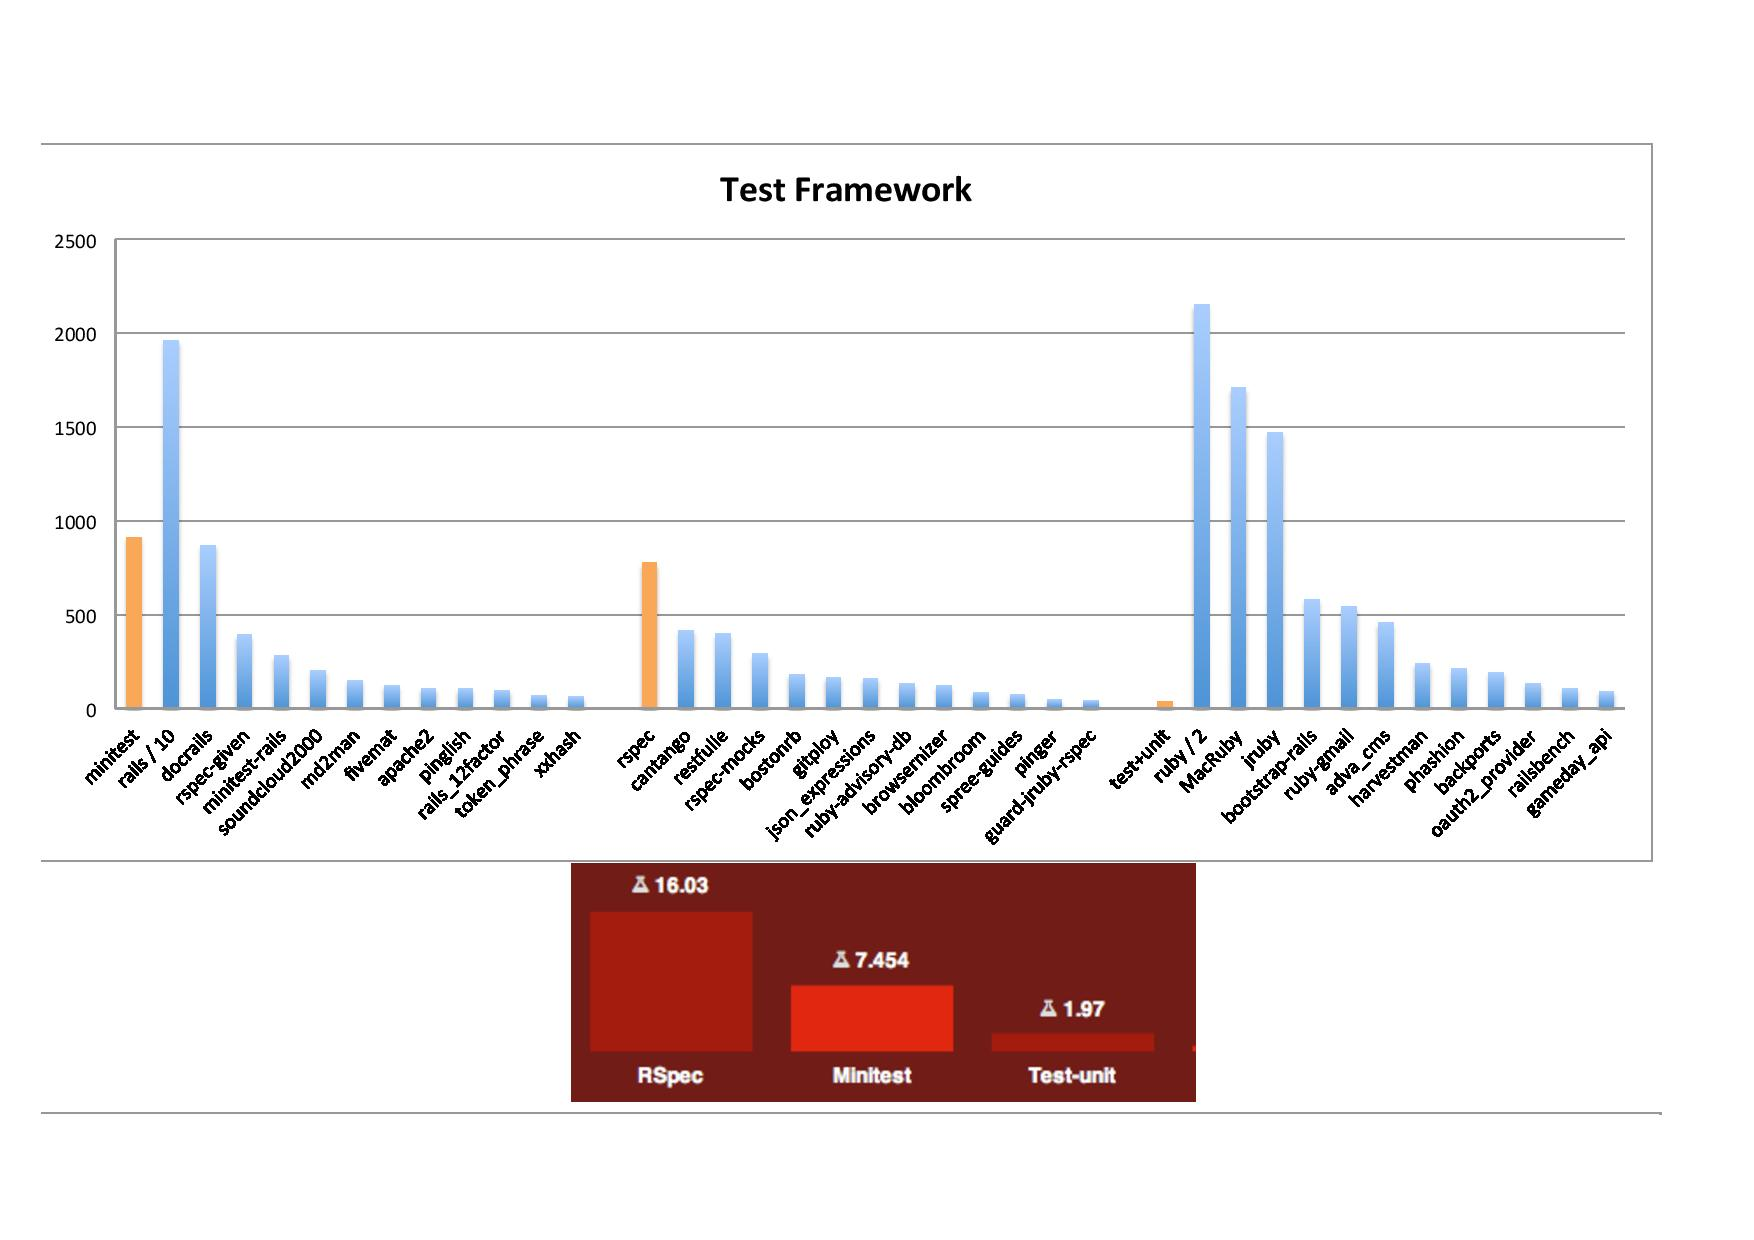
\includegraphics[width=15cm]{Imagens/gems-1.jpg}
	\caption*{Fonte: GitHub API e Ruby Toolbox (2013)}
\end{figure}
\begin{figure}[ht]
	\centering
    \caption{Rails \textit{Uploaders}}
    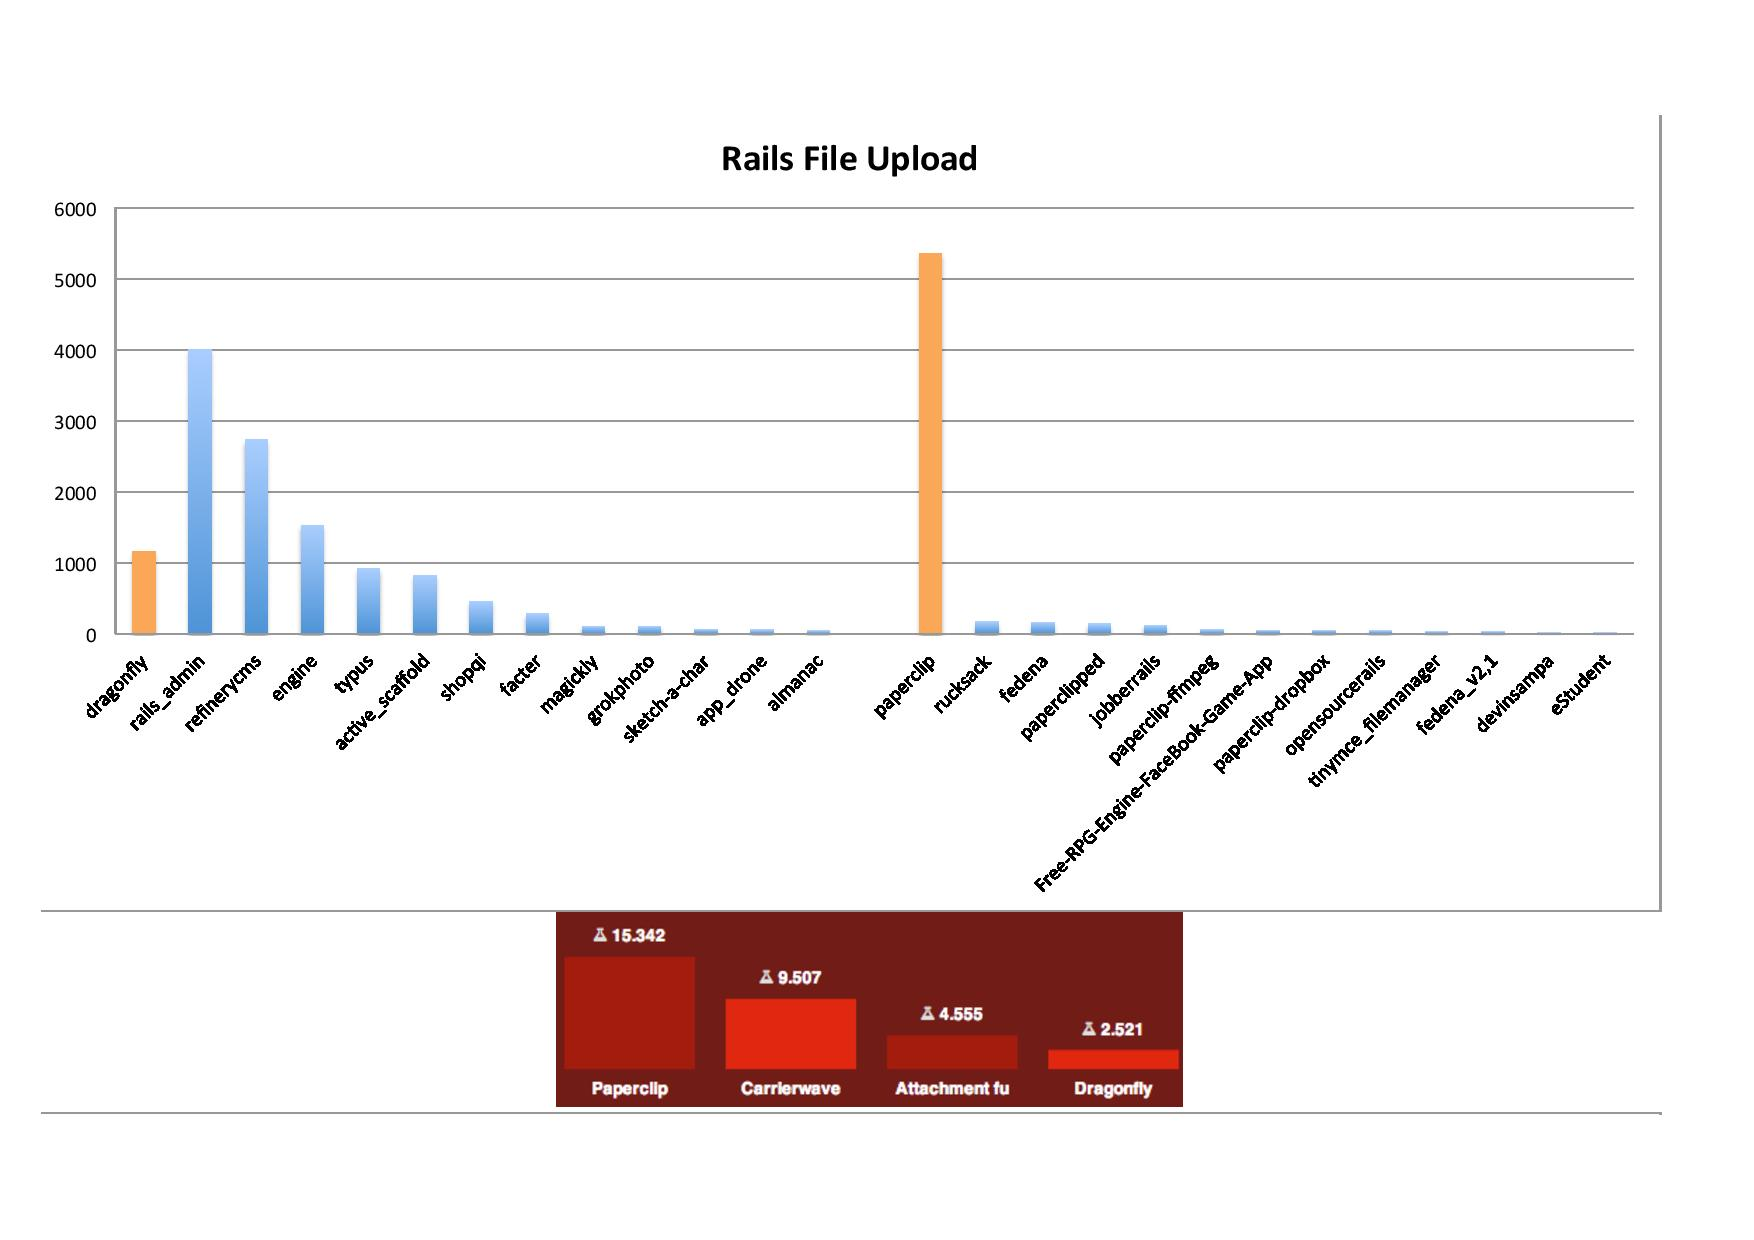
\includegraphics[width=15cm]{Imagens/gems-2.jpg}
	\caption*{Fonte: GitHub API e Ruby Toolbox (2013)}
\end{figure}
\begin{figure}[ht]
	\centering
    \caption{Clientes HTTP}
    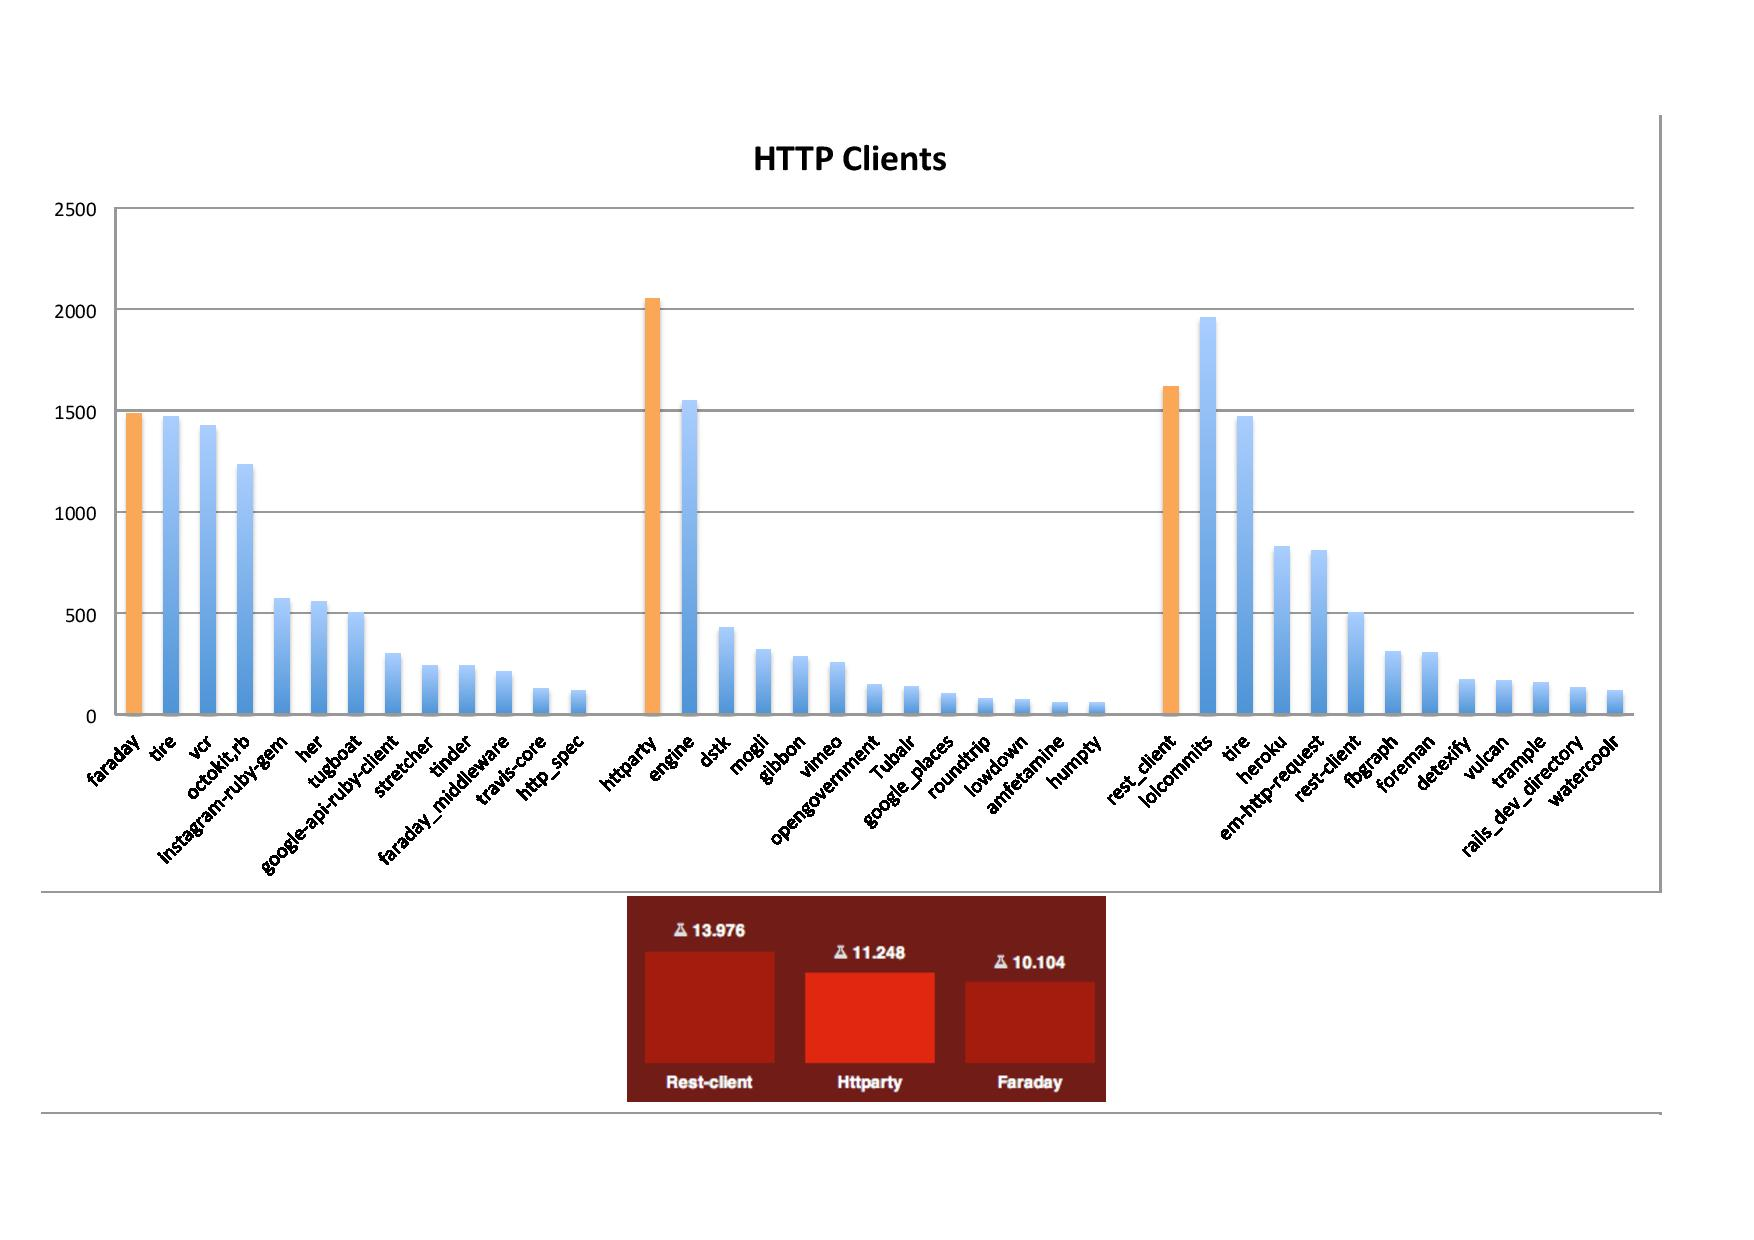
\includegraphics[width=15cm]{Imagens/gems-3.jpg}
	\caption*{Fonte: GitHub API e Ruby Toolbox (2013)}
\end{figure}
\begin{figure}[ht]
	\centering
    \caption{Construtores de Formulários}
    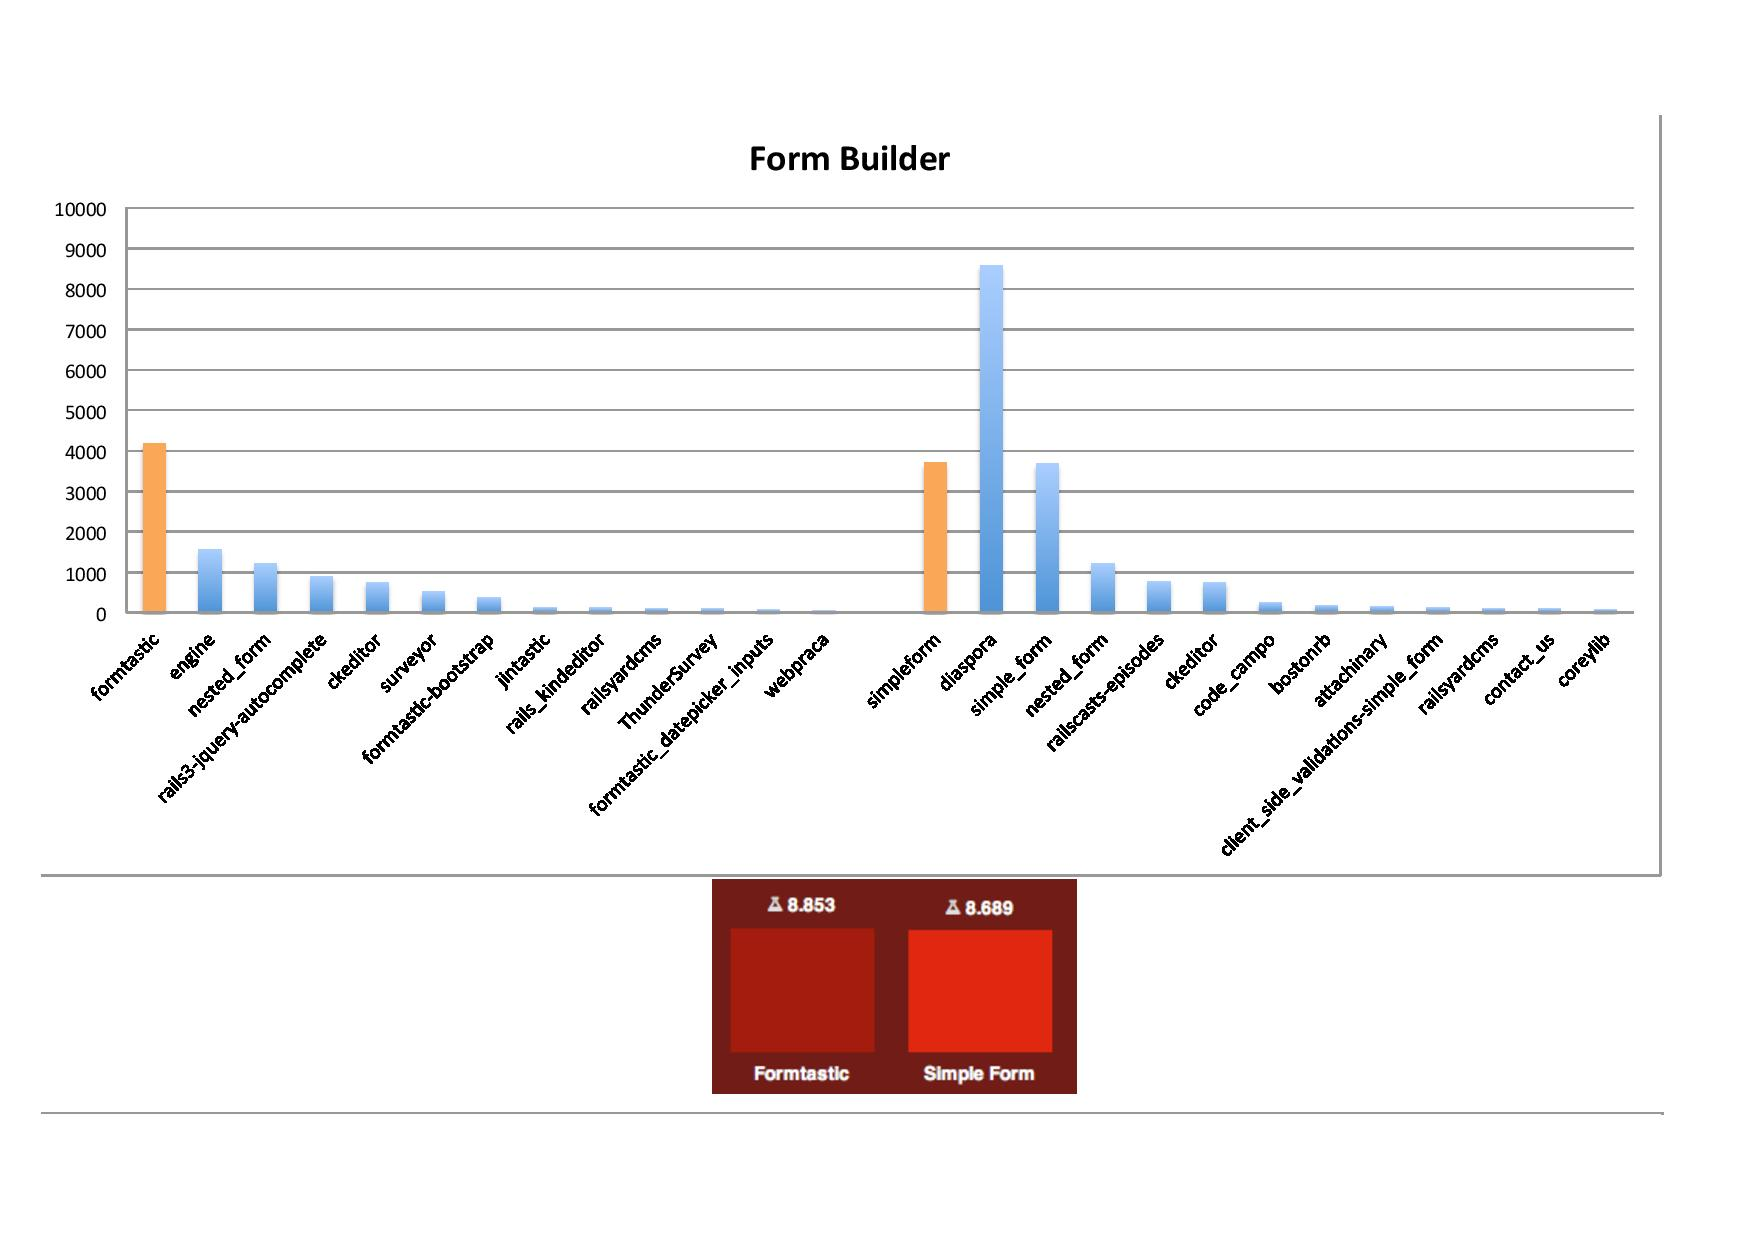
\includegraphics[width=15cm]{Imagens/gems-4.jpg}
	\caption*{Fonte: GitHub API e Ruby Toolbox (2013)}
\end{figure}
\begin{figure}[ht]
	\centering
    \caption{Interpretador de JSON}
    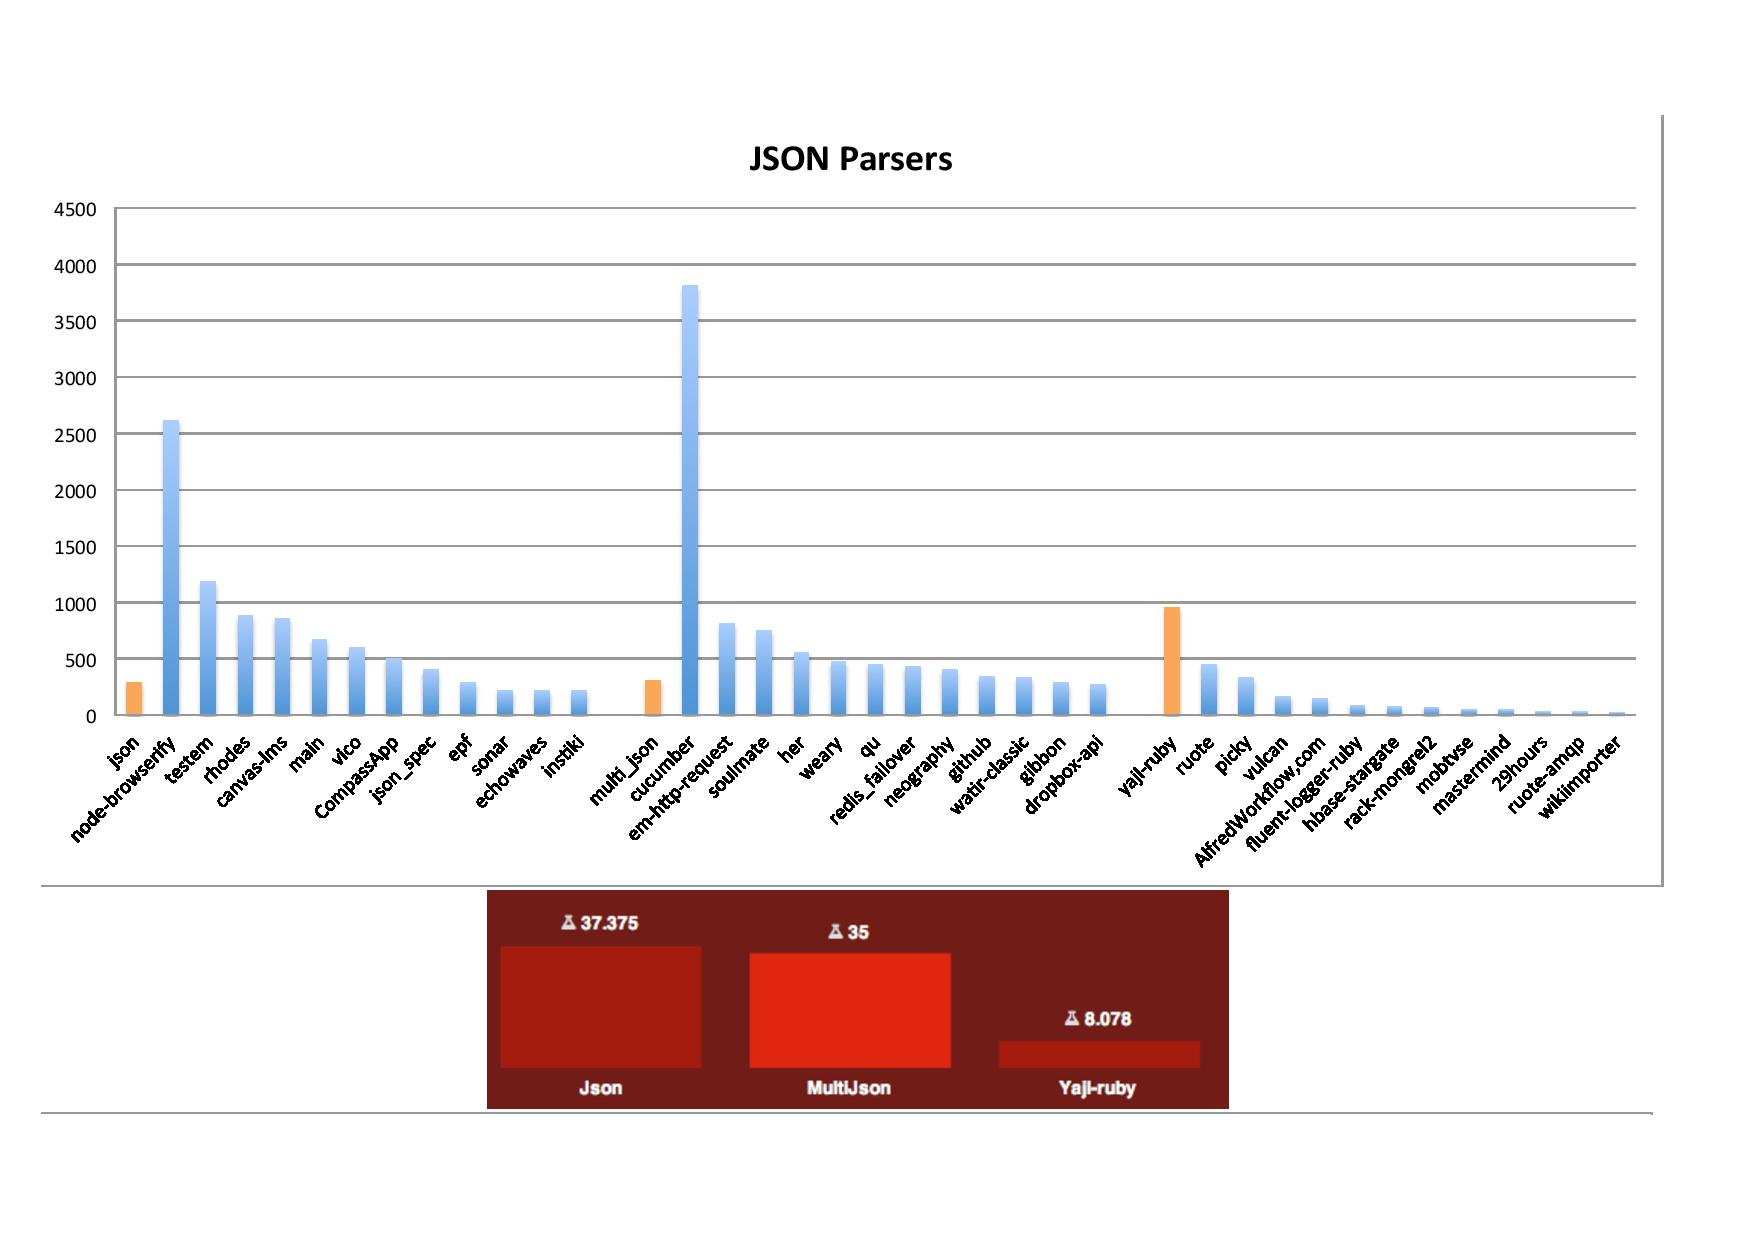
\includegraphics[width=15cm]{Imagens/gems-5.jpg}
	\caption*{Fonte: GitHub API e Ruby Toolbox (2013)}
\end{figure}
\begin{figure}[ht]
	\centering
    \caption{\textit{Template Engine}}
    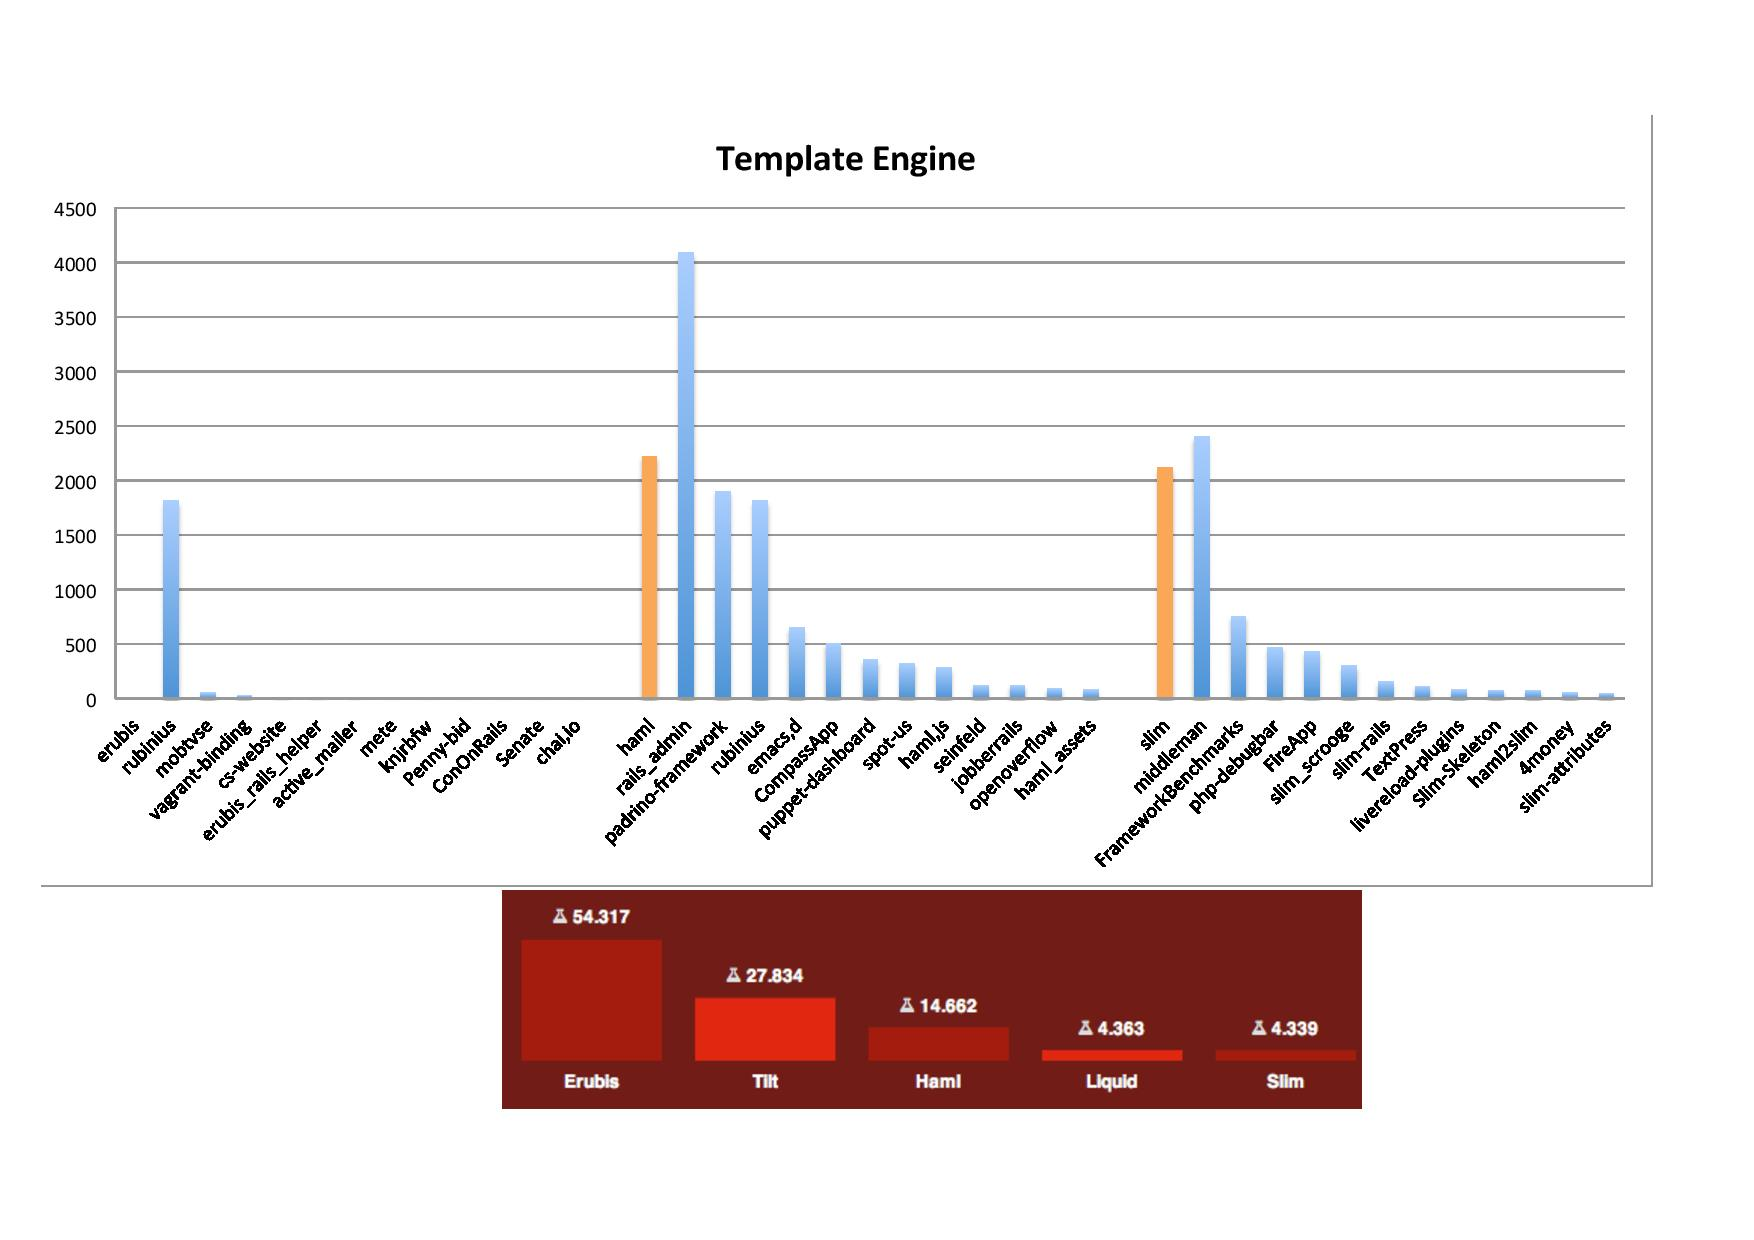
\includegraphics[width=15cm]{Imagens/gems-6.jpg}
	\caption*{Fonte: GitHub API e Ruby Toolbox (2013)}
\end{figure}
    
  	\include{Includes/ApendiceB}

	\bibliography{Capitulos/Referencias}
    
	\bibliographystyle{abnt-alf}

	\newpage

\end{document}